\documentclass[a4paper,fontset=windows]{ctexart}
\usepackage{amsmath,amssymb,bm}
\usepackage{anyfontsize,wasysym}
\allowdisplaybreaks
\usepackage{graphicx}
\usepackage[shortlabels]{enumitem}
\usepackage{indentfirst}
\setlength{\parindent}{0em}
\usepackage{geometry}
\geometry{top=3cm,bottom=3cm,left=2cm,right=2cm}
\usepackage{tikz}
\usetikzlibrary{arrows.meta,decorations.pathmorphing,decorations.pathreplacing,shapes}

\begin{document}

    \title{\textbf{理论力学作业}}
    \author{}
    \date{}

    \maketitle

    \section*{有心运动}

    \begin{itemize}

    \item[2.1]
    设地心为O点，地球质量为$M_\oplus$，半径为$R_\oplus$，在地球赤道处A点以仰角$\theta = 45^\circ$，初速度为第一宇宙速度的一半发射一物体，求该物体以OA为极轴的轨道方程。
    \begin{center}
        \begin{tikzpicture}[>=Stealth]
            \draw [->] (0,0) -- (4,0);
            \draw (0,0) circle [radius=3cm];
            \draw [->] (3,0) -- (4,1);
            \fill (0,0) circle [radius=2pt];
            \fill (3,0) circle [radius=2pt];
            \draw (-0.25,-0.25) node {O};
            \draw (3.25,-0.25) node {A};
            \draw [dashed] (3,0) -- (3,1);
            \draw (3.3535534,0.3535534) arc [start angle=45,end angle=90,radius=0.5cm];
            \draw (3.25,0.75) node {$\theta$};
        \end{tikzpicture}
    \end{center}

    \item[2.3]
    把地球和金星绕太阳（质量为$M_{\astrosun}$）运动的轨道都近似看成在同一平面的圆形，半径分别为$R$和$0.7R$，现在从地面发射一个如图中轨道所示的探测器去考察金星，发射速度最小为多少？
    \begin{center}
        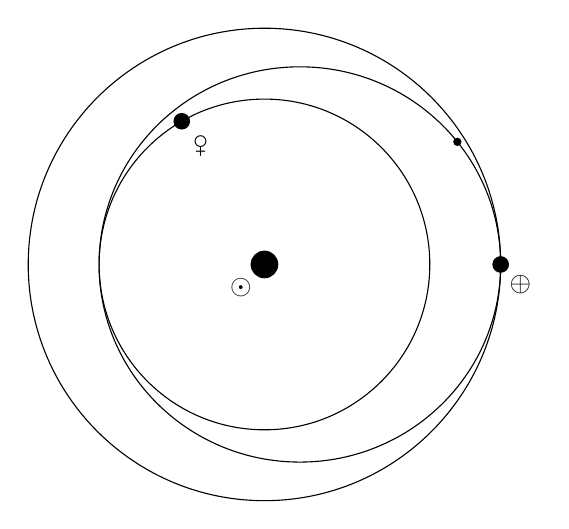
\begin{tikzpicture}[>=Stealth]
            \draw (0,0) circle [radius=3cm];
            \draw (0,0) circle [radius=2.1cm];
            \fill (0,0) circle [radius=5pt];
            \fill (3,0) circle [radius=3pt];
            \fill (-1.05,1.818653) circle [radius=3pt];
            \draw (0.45,0) ellipse [x radius=2.55cm,y radius=2.51cm];
            \fill (2.45,1.557102) circle [radius=1.5pt];
            \draw (-0.3,-0.3) node {\astrosun};
            \draw (3.25,-0.25) node {$\oplus$};
            \draw (-0.8,1.5) node {\venus};
        \end{tikzpicture}
    \end{center}

    \item[2.5]
    完全相同的小球组成的均匀、平行射束从远处以初速度$v_0$射向月球（质量为$M_{\!\!\rightmoon}$），求能击中月球表面的碰撞总截面的大小，用月球半径$a$、月球的逃逸速度$u$和$v_0$表示。

    \end{itemize}

    \section*{小振动}

    \begin{itemize}

    \item[3.1]
    两质点由三个弹簧连接，在同一直线上运动。质点的质量都是$m$，弹簧的自然长度和劲度系数都分别是$l_0$和$k$，两个固定端点之间的距离为$3l_0$。 \\
    (1)求体系的小振动频率； \\
    (2)如果每个质点都带正电荷$q$，再求体系的小振动频率。
    \begin{center}
        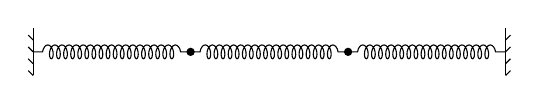
\begin{tikzpicture}[>=Stealth]
            \draw [decorate,decoration={coil,pre length=1.2mm,segment length=0.9mm,post length=1mm}] (0,0) -- (2,0);
            \draw [decorate,decoration={coil,pre length=1.2mm,segment length=0.9mm,post length=1mm}] (2,0) -- (4,0);
            \draw [decorate,decoration={coil,pre length=1.2mm,segment length=0.9mm,post length=1mm}] (4,0) -- (6,0);
            \draw [decorate,decoration={border,segment length=1.5mm,angle=45}] (0,-0.3) -- (0,0.3);
            \draw (0,-0.3) -- (0,0.3);
            \draw [decorate,decoration={border,segment length=1.5mm,angle=-45}] (6,-0.3) -- (6,0.3);
            \draw (6,-0.3) -- (6,0.3);
            \fill (2,0) circle [radius=1.5pt];
            \fill (4,0) circle [radius=1.5pt];
        \end{tikzpicture}
    \end{center}

    \item[3.2]
    一杆OA绕固定点O在竖直平面内摆动，另一杆AB绕A在同一竖直平面内运动。两杆的质量均为$m$，长度均为$l$。求双杆体系作小振动时的频率和运动。
    \begin{center}
        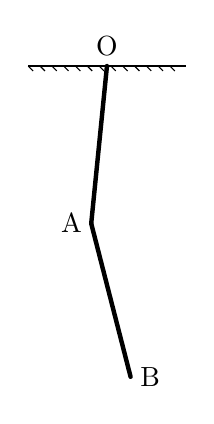
\begin{tikzpicture}[>=Stealth]
            \draw [decorate,decoration={border,segment length=1.5mm,angle=-45}] (0,0) -- (2,0);
            \draw (0,0) -- (2,0);
            \draw [ultra thick,line cap=round] (1,0) -- (0.8,-2);
            \draw [ultra thick,line cap=round] (0.8,-2) -- (1.3,-3.946792);
            \draw (1,0.25) node {O};
            \draw (0.55,-2) node {A};
            \draw (1.55,-3.946792) node {B};
        \end{tikzpicture}
    \end{center}

    \item[3.3]
    在两根自然长度为$l_0$，弹性系数为$k$的弹簧下端悬挂一根长度为$l$，质量为$m$的细棒，弹簧的悬挂点相距也为$l$。只考虑体系在竖直平面内因两弹簧的不同伸缩情况而运动。 \\
    (1)通过分析本征值问题求体系小振动的频率和运动； \\
    (2)通过分析简正模式，求本征频率和简正坐标。
    \begin{center}
        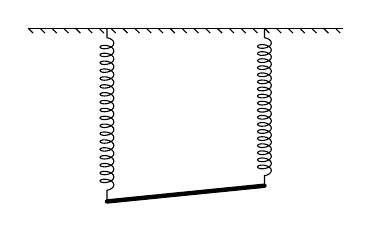
\begin{tikzpicture}[>=Stealth]
            \draw [decorate,decoration={border,segment length=1.5mm,angle=-45}] (0,0) -- (4,0);
            \draw (0,0) -- (4,0);
            \draw [decorate,decoration={coil,pre length=1.2mm,segment length=1mm,post length=1.2mm}] (1,0) -- (1,-2.2);
            \draw [decorate,decoration={coil,pre length=1.2mm,segment length=0.9mm,post length=1mm}] (3,0) -- (3,-2);
            \draw [ultra thick,line cap=round] (1,-2.2) -- (3,-2);
        \end{tikzpicture}
    \end{center}

    \item[3.4]
    如图所示的一维力学体系，处于平衡位置时，整个体系关于C对称。弹簧的劲度系数均为$k$，质点A、B的质量均为$m$，质点C的质量为$M$。 \\
    (1)取三个质点偏离平衡位置的坐标$x_1$、$x_2$、$x_3$为广义坐标，求小振动的频率。 \\
    (2)再取$x_2-x_1$和$x_3-x_2$为广义坐标，求小振动的频率。与(1)中结果比较，可以得出什么结论？
    \begin{center}
        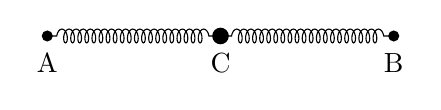
\begin{tikzpicture}[>=Stealth]
            \draw [decorate,decoration={coil,pre length=1.2mm,segment length=0.9mm,post length=1.2mm}] (0,0) -- (2.2,0);
            \draw [decorate,decoration={coil,pre length=1.4mm,segment length=0.9mm,post length=1mm}] (2.2,0) -- (4.4,0);
            \fill (0,0) circle [radius=2pt];
            \fill (2.2,0) circle [radius=3pt];
            \fill (4.4,0) circle [radius=2pt];
            \draw (0,-0.35) node {A};
            \draw (4.4,-0.35) node {B};
            \draw (2.2,-0.35) node {C};
        \end{tikzpicture}
    \end{center}

    \item[3.5]
    一个自由度为4的理想、完整、稳定约束的保守力学体系，广义坐标为$q_i(i=1,2,3,4)$，相应的势能和动能二次式的系数矩阵分别为：（$\omega_0>0$）
    \[
    \bm{V} =
        \begin{bmatrix}
            \omega_0^2 & 0 & 0 & 0 \\
            0 & \omega_0^2 & 0 & 0 \\
            0 & 0 & 2\omega_0^2 & -2\omega_0^2 \\
            0 & 0 & -2\omega_0^2 & 3\omega_0^2
        \end{bmatrix},\qquad
    \bm{T} =
        \begin{bmatrix}
            1 & 0 & 0 & 0 \\
            0 & 1 & 0 & 0 \\
            0 & 0 & 1 & -1 \\
            0 & 0 & -1 & 1
        \end{bmatrix}
    \]
    (1)求该体系的小振动解，并由求出的本征矢量判断哪几个广义坐标已经是简正坐标； \\
    (2)找出全部简正坐标，并求出其小振动解； \\
    (3)已知$\bm{T}$为无量纲的量，问$\bm{V}$和$q$的量纲是什么？ \\
    (4)在以上求出的四个$\omega$中，哪些是简并的，简并度是多少？（$\omega_1=\omega_2=\omega_3=\omega_0$，$\omega_4=\sqrt{2}\omega_0$）

    \end{itemize}

    \section*{刚体运动学}

    \begin{itemize}

    \item[4.2]
    半径为$a$的圆柱夹在互相平行的两块足够大的平板之间，两块板分别以$v_1$、$v_2$的速度反向运动。圆柱和板之间无滑动。 \\
    (1)求此时圆柱瞬心的位置； \\
    (2)求圆柱与上板的接触点A的加速度（A点是圆柱上的点）。
    \begin{center}
        \begin{tikzpicture}[>=Stealth]
            \node [draw,rectangle,minimum height=0.5cm,minimum width=6cm] at (0,2.25) {};
            \node [draw,rectangle,minimum height=0.5cm,minimum width=6cm] at (0,-2.25) {};
            \draw (0,0) circle [radius=2cm];
            \fill (0,0) circle [radius=2pt];
            \draw (-0.25,-0.25) node {O};
            \fill (0,2) circle [radius=2pt];
            \draw (0,1.75) node {A};
            \draw [dashed,->] (0,0) -- (1.41421356,1.41421356);
            \draw (1,0.7) node {$a$};
            \draw [->] (3.5,2.25) -- (4.5,2.25);
            \draw (4,2.5) node {$v_1$};
            \draw [<-] (-4.5,-2.25) -- (-3.5,-2.25);
            \draw (-4,-2.5) node {$v_2$};
        \end{tikzpicture}
    \end{center}

    \item[4.3]
    一半径为$a$的圆盘O以角速度$\omega$绕其中心转动，另一半径为$b$的圆盘$\mathrm{O}'$以角速度$\omega'$在大圆外纯滚动（即两圆盘接触点不发生滑动）。 \\
    (1)证明：两圆连心线$\mathrm{OO}'$转动的角速度为：
    \[
    \varOmega=\dfrac{a\omega+b\omega'}{a+b}
    \]
    (2)求圆$\mathrm{O}'$在圆O上滚一周又回到与圆O上的同一起点相接触所需的时间$t_1$； \\
    (3)求圆$\mathrm{O}'$回到空间原来位置所需的时间$t_2$。
    \begin{center}
        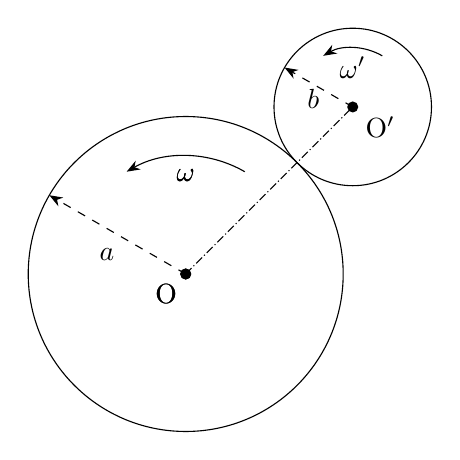
\begin{tikzpicture}[>=Stealth]
            \draw (0,0) circle [radius=2cm];
            \fill (0,0) circle [radius=2pt];
            \draw (-0.25,-0.25) node {O};
            \draw (2.12132,2.12132) circle [radius=1cm];
            \fill (0,0) circle [radius=2pt];
            \draw (-0.25,-0.25) node {O};
            \fill (2.12132,2.12132) circle [radius=2pt];
            \draw (2.47132,1.87132) node {$\mathrm{O}'$};
            \draw [densely dash dot] (0,0) -- (2.12132,2.12132);
            \draw [dashed,->] (0,0) -- (-1.73205,1);
            \draw (-1,0.25) node {$a$};
            \draw [dashed,->] (2.12132,2.12132) -- (1.255295,2.62132);
            \draw (1.62132,2.22132) node {$b$};
            \draw (0,1.25) node {$\omega$};
            \draw [->] (0.75,1.29904) arc [start angle=60,end angle=120,radius=1.5cm];
            \draw (0,1.25) node {$\omega$};
            \draw [->] (2.49632,2.77084) arc [start angle=60,end angle=120,radius=0.75cm];
            \draw (2.12132,2.62132) node {$\omega'$};
        \end{tikzpicture}
    \end{center}

    \item[4.4]
    高为$h$，顶角为$2\alpha$的圆锥在一平面上作纯滚动。已知此锥轴线以等角速度$\bm{\omega}$绕$z$轴旋转，规定$\bm{\omega}$方向竖直向上，即沿$+z$方向。 \\
    (1)此锥体运动角速度$\bm{\varOmega}$（圆锥旋转的唯一角速度，即公转、自转叠加后的角速度）的大小和方向； \\
    (2)锥体底面最高点A的速度$\bm{v}_A$和加速度$\bm{a}_A$； \\
    (3)总的角加速度$\bm{\beta}=\dot{\bm{\varOmega}}$。
    \begin{center}
        \begin{tikzpicture}[>=Stealth]
            \draw [->] (0,0) -- (3.444093,-1);
            \draw (0,0) -- (2.563457,0.74499);
            \draw (2.598076,0) ellipse [x radius=0.3cm,y radius=0.75cm];
            \draw [dashed] (0,0) -- (2.598076,0);
            \draw [dashed] (2.598076,0) -- (2.598076,0.75);
            \draw (2.725,0.375) node {$h$};
            \draw (1.325,0) arc [start angle=0,end angle=16.204875,radius=1.325cm];
            \draw (1.525,0.25) node {$\alpha$};
            \draw [->] (0,0) -- (0,4);
            \draw [->] (0,0) -- (-3.444093,-1);
            \draw [->] (0.5,0.75) arc [start angle=0,end angle=300,x radius=0.5cm,y radius=0.3cm];
            \draw (0.25,1.25) node {$\bm{\omega}$};
            \fill (2.598076,0.75) circle [radius=1.5pt];
            \draw (2.598076,1) node {A};
            \draw (0,-0.25) node {O};
            \draw (-3.25,-1.25) node {$x$};
            \draw (3.25,-1.25) node {$y$};
            \draw (0.25,3.75) node {$z$};
        \end{tikzpicture}
    \end{center}

    \end{itemize}

    \section*{刚体动力学}

    \begin{itemize}

    \item[5.2]
    若刚体对某点的主转动惯量$I_1=I_2\neq I_3$，即其惯量椭球为旋转椭球，证明此刚体绕该点运动时角动量$\bm{J}$、角速度$\bm{\omega}$和$z$轴一定在同一平面上，并讨论哪个量在中间。

    \item[5.4]
    一个平面摆由长度为$l$、质量为$m$的均匀细杆和半径为$a$、质量为$M$的均匀薄圆盘铰接而成，圆盘可以在其竖直平面内自由摆动。求这个摆运动的运动方程。
    \begin{center}
        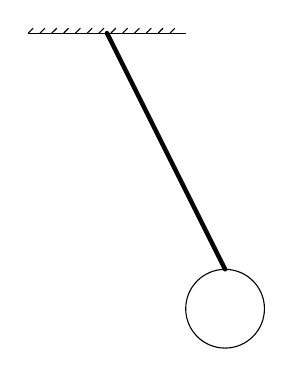
\begin{tikzpicture}[>=Stealth]
            \draw [decorate,decoration={border,segment length=1.5mm,angle=45}] (-1,0) -- (1,0);
            \draw (-1,0) -- (1,0);
            \draw [ultra thick,line cap=round] (0,0) -- (1.5,-3);
            \draw (1.5,-3.5) circle [radius=0.5cm];
        \end{tikzpicture}
    \end{center}

    \item[5.9]
    一个旋转对称的刚体（$I_1=I_2$）受外力作用而绕对称轴上一点作正规进动。已知自转角速度为$\varOmega_1$，进动角速度为$\varOmega_2$，章动角为$\theta$。用角动量定理导出该刚体对固定点总外力矩的公式为：
    \[
    \bm{N} = I_3 \cdot (\bm{\varOmega}_2\times\bm{\varOmega}_1) \cdot \left(1 + \frac{I_3-I_1}{I_3}\cdot\frac{\varOmega_2}{\varOmega_1}\cos\theta\right)
    \]

    \item[5.10]
    有一块匀质长方形薄板，边长分别为为$a$、$b$（$a>b$），质量为$m$，以匀角速度$\omega_0$绕其对角线AB转动。求其顶点A和B处的轴承上所受到的作用力。
    \begin{center}
        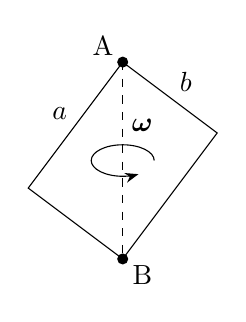
\begin{tikzpicture}[>=Stealth]
            \node [draw,rectangle,minimum height=1.5cm,minimum width=2cm,rotate=53.130102] at (0,0) {};
            \fill (0,1.25) circle [radius=2pt];
            \fill (0,-1.25) circle [radius=2pt];
            \draw [dashed] (0,1.25) -- (0,-1.25);
            \draw (-0.25,1.45) node {A};
            \draw (0.25,-1.45) node {B};
            \draw (-0.8,0.6) node {$a$};
            \draw (0.8,1) node {$b$};
            \draw [->] (0.4,0) arc [start angle=0,end angle=300,x radius=0.4cm,y radius=0.2cm];
            \draw (0.25,0.45) node {$\bm{\omega}$};
        \end{tikzpicture}
    \end{center}

    \end{itemize}

    \section*{正则方程}

    \begin{itemize}

    \item[6.1]
    若由变量$(q,p)$变换为$(\dot{p},p)$，特征函数相应地由$H(q,p,t)$变换为$L'(\dot{p},p.t)$。按照Legendre变换有：
    \[
    L'(\dot{p},p.t) = H(q,p,t) + \dot{p}q,\quad \dot{p}=-\frac{\partial H}{\partial q}
    \]
    证明由正则方程推出用$L'(\dot{p},p.t)$表示的运动方程为：
    \[
    \frac{\mathrm{d}}{\mathrm{d}t}\left(\frac{\partial L'}{\partial \dot{p}}\right) - \frac{\partial L'}{\partial p} = 0
    \]

    \item[6.2]
    质点$m$在两个弹簧的作用下作直线运动。设两固定点之间的距离为$a$，两个弹簧的弹性系数分别为$k_1$和$k_2$。写出质点的Lagrange函数和Hamilton函数，列出正则方程并求解。
    \begin{center}
        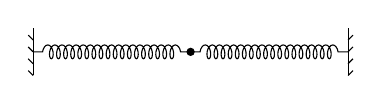
\begin{tikzpicture}[>=Stealth]
            \draw [decorate,decoration={coil,pre length=1.2mm,segment length=0.9mm,post length=1mm}] (0,0) -- (2,0);
            \draw [decorate,decoration={coil,pre length=1.2mm,segment length=0.9mm,post length=1mm}] (2,0) -- (4,0);
            \draw [decorate,decoration={border,segment length=1.5mm,angle=45}] (0,-0.3) -- (0,0.3);
            \draw (0,-0.3) -- (0,0.3);
            \draw [decorate,decoration={border,segment length=1.5mm,angle=-45}] (4,-0.3) -- (4,0.3);
            \draw (4,-0.3) -- (4,0.3);
            \fill (2,0) circle [radius=1.5pt];
        \end{tikzpicture}
    \end{center}

    \item[6.3]
    设单摆（摆长为$l$，摆锤质量为$m$）的悬点只能沿抛物线$z=ax^2$运动，写出系统的Hamilton函数。
    \begin{center}
        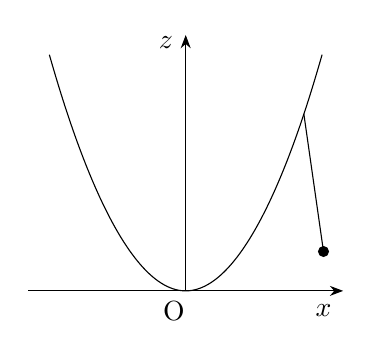
\begin{tikzpicture}[>=Stealth]
        \draw (-1.732051,3) parabola bend (0,0) (1.732051,3);
        \draw [->] (-2,0) -- (2,0);
        \draw [->] (0,0) -- (0,3.25);
        \draw (1.5,2.25) -- (1.75,0.5);
        \fill (1.75,0.5) circle [radius=2pt];
        \draw (-0.15,-0.25) node {O};
        \draw (1.75,-0.25) node {$x$};
        \draw (-0.25,3.15) node {$z$};
        \end{tikzpicture}
    \end{center}

    \item[6.5]
    在有心力势$V(\rho)$作用下，一带电粒子（质量为$m$，电荷量为$e$）作平面运动。又垂直于此平面加一均匀恒定磁场$\bm{B}_0$，其磁矢势为：$\bm{A}=\dfrac{1}{2}\bm{B}_0\times\bm{r}$。 \\
    (1)写出粒子的Hamilton函数； \\
    (2)以角速度$\bm{\omega}=-\dfrac{e}{2m}\bm{B}_0$转动的坐标系里的坐标为广义坐标，求粒子的Hamilton函数。

    \item[6.6]
    对于一个质量为$m$的质点在势场$V(r)=-\dfrac{GM}{r}$中做Kepler运动，可以定义Laplace-Runge-Lenz矢量（又称偏心率矢量）：
    \[
    \bm{e} = \frac{1}{GMm^2}\bm{p}\times\bm{J}-\frac{\bm{r}}{r}
    \]
    (1)证明$[\bm{e},H]=0$，由此说明该矢量守恒； \\
    (2)由$\bm{e}\cdot\bm{r}$求轨道方程，并证明$\bm{e}$取由力心到近日点的方向，大小等于偏心率$e$。该矢量守恒使得近力心点方向不变，从而保证了椭圆轨道闭合。
    \end{itemize}

    \section*{力学变分原理}

    \begin{itemize}

    \item[6.5]
    证明下列变换为正则变换。 \\
    (1)变换：
    \[
    Q=\ln\left(\dfrac{1}{q}\sin p\right),\quad P=q\cot p
    \]
    (2)变换：
    \[
        q=\sqrt{\dfrac{2Q}{k}}\cos P,\quad p=\sqrt{2Qk}\sin P
    \]

    \end{itemize}
\end{document}
